\documentclass[14pt, table]{extarticle}
\usepackage{amsfonts}
\usepackage{amsmath}
\usepackage[utf8]{inputenc}
\usepackage[a4paper, total={7in, 10.5in}]{geometry}
\usepackage[table]{xcolor}
\usepackage{tgbonum}
\usepackage{float}
\usepackage{graphicx}
\graphicspath{ {./images/} }
\DeclareGraphicsExtensions{.png,.jpg}
\usepackage{caption}
\usepackage{tikz}
\usepackage{circuitikz}
\usepackage[T1]{fontenc}
\usetikzlibrary{quotes,angles}
\usetikzlibrary{arrows}
\usetikzlibrary{circuits.logic.US}
\usetikzlibrary{positioning}
\hyphenpenalty 5000
\usepackage{subfig}
\usepackage{array}

\title{\textbf{Dodatek do sprawozdania} \\ \Large{Ćwiczenie 4.5}}
\date{10 maja 2023}
\author{ \Large{Jan Kwinta, grupa 12}}

\newcommand{\nl}{\vspace{0.5cm}}
\newcommand{\nz}{\vspace{1.5cm}}

\begin{document}
\maketitle

Żeby nieco rozszerzyć materiał postanowiłem zaprojektować pełną logikę wyświetlacza siedmiosegmentowego (a nie tylko jednego segmentu, jak w zadaniu 5). Na kolejnych stronach zamieściłem pełny schemat układu logicznego oraz notatki z obliczeń poszczególnych funkcji logicznych z minimalizacją metodą Karnaugha. \\

Zdaję sobie sprawę że nie jest to najbardziej optymalna implementacja. Moim celem było to, aby układ każdego segmentu dało się zbudować używając jednego układu 7400 i jednego układu 7402; czyli korzystając z co najwyżej 4 bramek NAND i co najwyżej 4 bramek NOR. Niestety, do zbudowania funkcji logicznej segmentu \textit{d} potrzebowałem użyć czterech bramek NAND i pięciu bramek NOR. \\

Oczywiście nie miałem czasu przetestować mojego schematu na prawdziwych układach w pracowni elektronicznej, ale skonstruowałem go w programie umożliwiającym symulację bramek logicznych i wyświetlacz działał poprawnie. \\

Przyjmujemy, że otrzymujemy na wejściu liczbę binarną. Wyświetlacz ma wyświetlić ją jako liczbę ósemkową. Każdą trójkę bitów przetwarzamy osobno jako $(A, B, C)$, gdzie A jest najmłodszym, a C najstarszym bitem. Dla wygody na wejściu dostajemy także trójkę $(\overline{A}, \overline{B}, \overline{C})$ będącą zaprzeczeniami odpowiednich bitów. Jeżeli komuś bardzo zależy, żeby układ działał wyłącznie na bramkach NAND i NOR to zaprzeczenia możemy realizować na nich, tak jak w zadaniu 4.3.

\newpage

\begin{center}
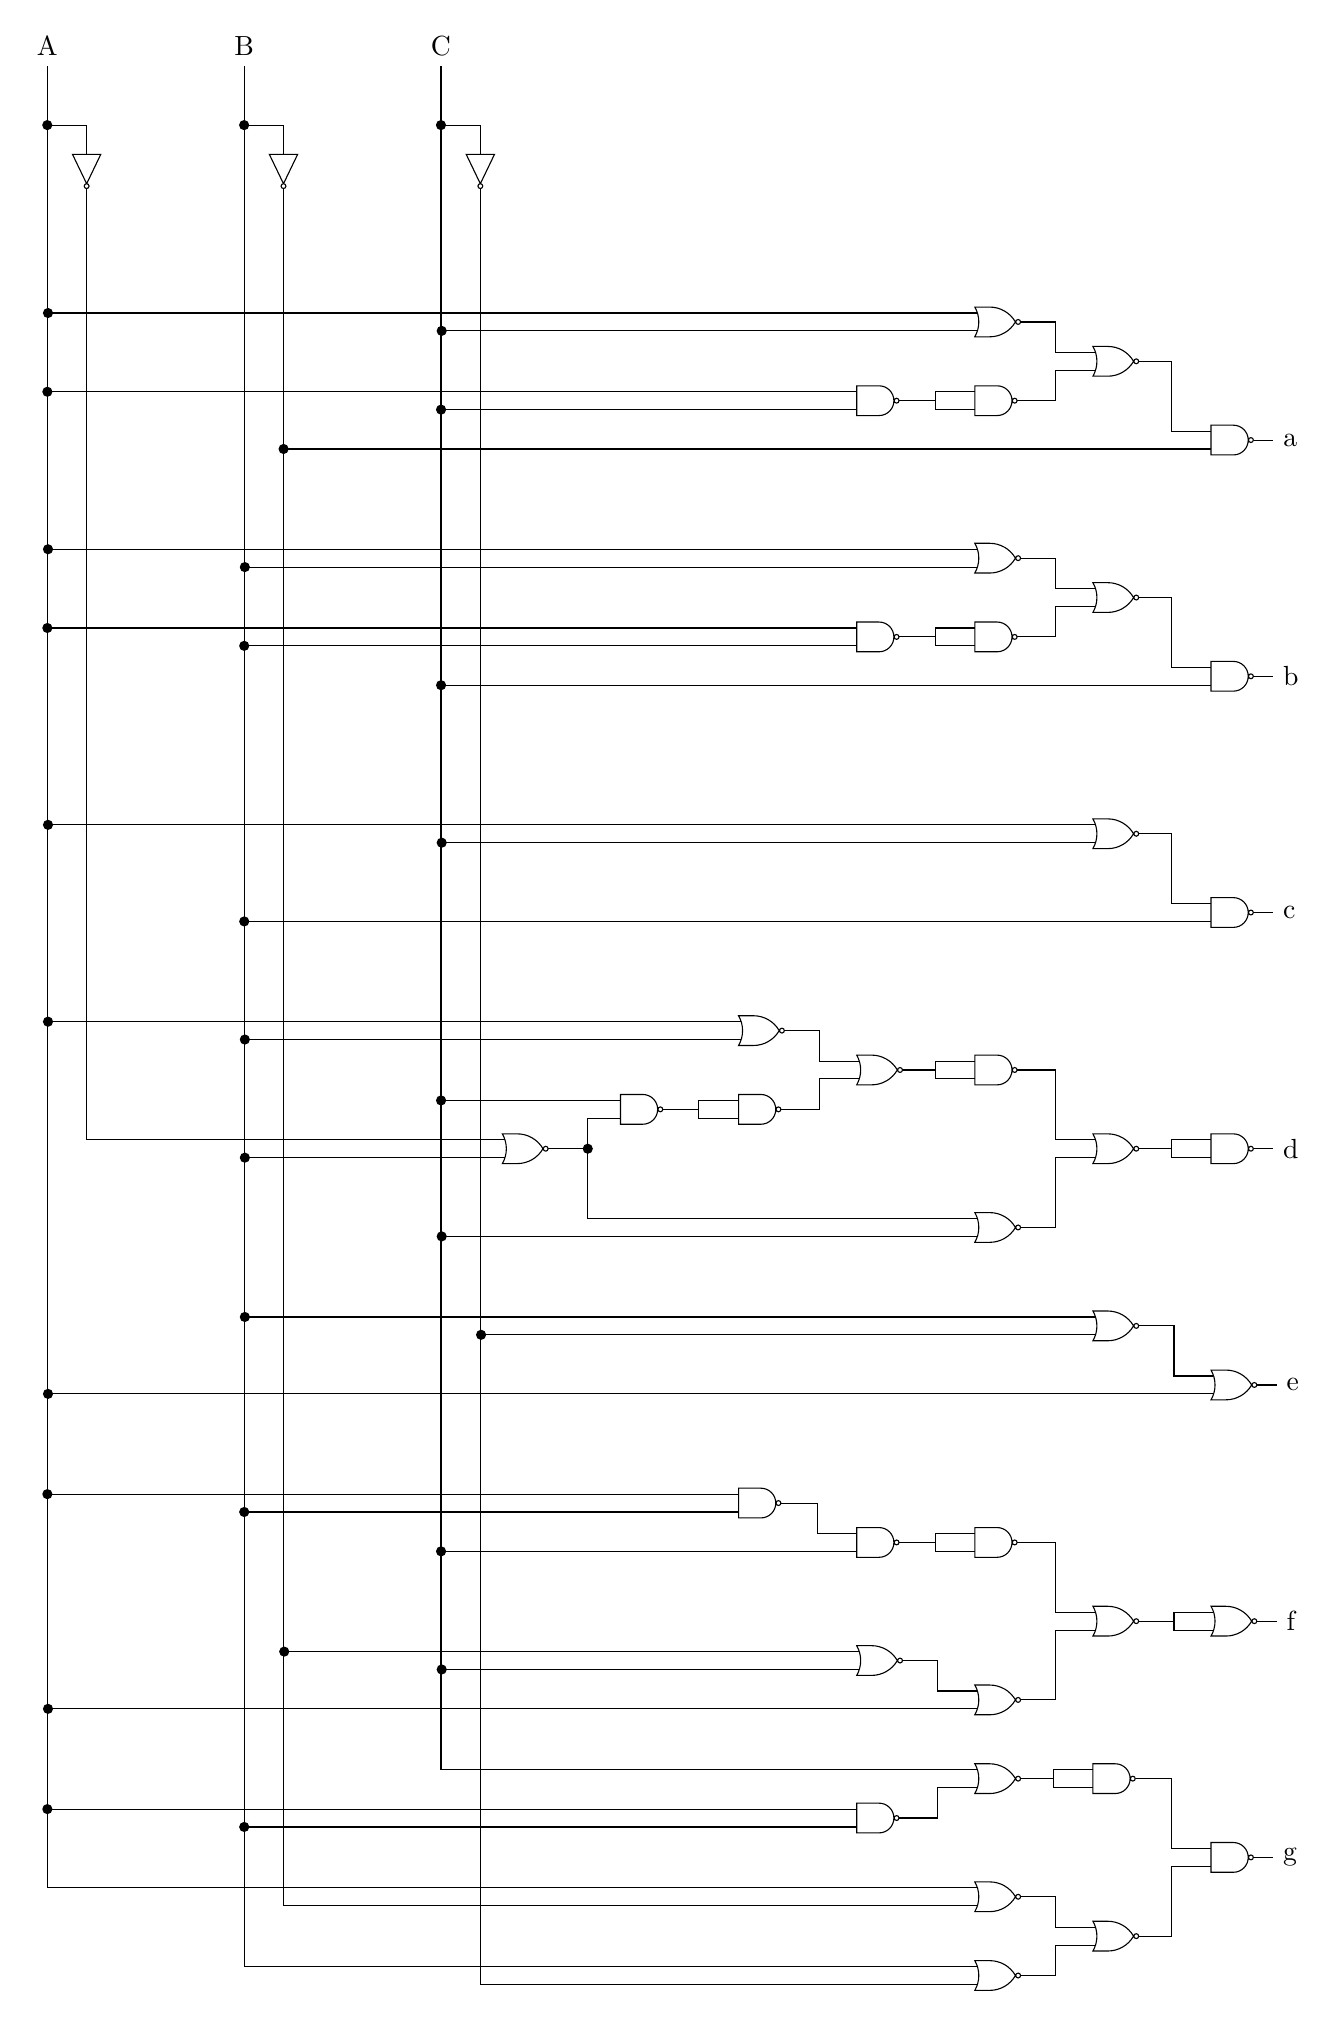
\begin{tikzpicture}[circuit logic US, scale = 0.5]

	\node (A) at (0, 0) {A};
	\node (B) at (5, 0) {B};
	\node (C) at (10, 0) {C};

	\node [rotate=270, not gate] (notA) at (1, -3) {};
	\node [rotate=270, not gate] (notB) at (6, -3) {};
	\node [rotate=270, not gate] (notC) at (11, -3) {};

	\draw (notA.input) |- node [at end, circle, fill, inner sep=1.3pt]{} (0, -2);
	\draw (notB.input) |- node [at end, circle, fill, inner sep=1.3pt]{} (5, -2);
	\draw (notC.input) |- node [at end, circle, fill, inner sep=1.3pt]{} (10, -2);

	\node [nand gate, inputs=nnnn] (Anand1) at (30, -10) {};
	\node [nand gate, inputs=nnnn] (Bnand1) at (30, -16) {};
	\node [nand gate, inputs=nnnn] (Cnand1) at (30, -22) {};
	\node [nand gate, inputs=nnnn] (Dnand1) at (30, -28) {};
	\node [nor gate, inputs=nnnn] (Enor1) at (30, -34) {};
	\node [nor gate, inputs=nnnn] (Fnor1) at (30, -40) {};
	\node [nand gate, inputs=nnnn] (Gnand1) at (30, -46) {};

	\draw (Anand1.output) -- node[at end, right]{a} ++(right: 5mm);
	\draw (Bnand1.output) -- node[at end, right]{b} ++(right: 5mm);
	\draw (Cnand1.output) -- node[at end, right]{c} ++(right: 5mm);
	\draw (Dnand1.output) -- node[at end, right]{d} ++(right: 5mm);
	\draw (Enor1.output) -- node[at end, right]{e} ++(right: 5mm);
	\draw (Fnor1.output) -- node[at end, right]{f} ++(right: 5mm);
	\draw (Gnand1.output) -- node[at end, right]{g} ++(right: 5mm);


	\draw (Anand1.input 4) -- node [at end, circle, fill, inner sep=1.3pt]{} ++(left: 23.55); 
	\node [nor gate, inputs=nnnn] (Anor1) at (27, -8) {};
	\node [nor gate, inputs=nnnn] (Anor2) at (24, -7) {};
	\node [nand gate, inputs=nnnn] (Anand2) at (24, -9) {};
	\node [nand gate, inputs=nnnn] (Anand3) at (21, -9) {};
	\draw (Anor1.input 1) -- ++(left: 1) |- (Anor2.output);
	\draw (Anor1.input 4) -- ++(left: 1) |- (Anand2.output);
	\draw (Anand1.input 1) -- ++(left: 1) |- (Anor1.output);
	\draw (Anand2.input 1) -- ++(left: 1) |- (Anand3.output);
	\draw (Anand2.input 4) -- ++(left: 1) |- (Anand3.output);
	\draw (Anor2.input 1) -- node [at end, circle, fill, inner sep=1.3pt]{} ++(left: 23.6);
	\draw (Anor2.input 4) -- node [at end, circle, fill, inner sep=1.3pt]{} ++(left: 13.6);
	\draw (Anand3.input 1) -- node [at end, circle, fill, inner sep=1.3pt]{} ++(left: 20.55);
	\draw (Anand3.input 4) -- node [at end, circle, fill, inner sep=1.3pt]{} ++(left: 10.55);


	\draw (Bnand1.input 4) -- node [at end, circle, fill, inner sep=1.3pt]{} ++(left: 19.55); 
	\node [nor gate, inputs=nnnn] (Bnor1) at (27, -14) {};
	\node [nor gate, inputs=nnnn] (Bnor2) at (24, -13) {};
	\node [nand gate, inputs=nnnn] (Bnand2) at (24, -15) {};
	\node [nand gate, inputs=nnnn] (Bnand3) at (21, -15) {};
	\draw (Bnor1.input 1) -- ++(left: 1) |- (Bnor2.output);
	\draw (Bnor1.input 4) -- ++(left: 1) |- (Bnand2.output);
	\draw (Bnand1.input 1) -- ++(left: 1) |- (Bnor1.output);
	\draw (Bnand2.input 1) -- ++(left: 1) |- (Bnand3.output);
	\draw (Bnand2.input 4) -- ++(left: 1) |- (Bnand3.output);
	\draw (Bnor2.input 1) -- node [at end, circle, fill, inner sep=1.3pt]{} ++(left: 23.6);
	\draw (Bnor2.input 4) -- node [at end, circle, fill, inner sep=1.3pt]{} ++(left: 18.6);
	\draw (Bnand3.input 1) -- node [at end, circle, fill, inner sep=1.3pt]{} ++(left: 20.55);
	\draw (Bnand3.input 4) -- node [at end, circle, fill, inner sep=1.3pt]{} ++(left: 15.55);


	\draw (Cnand1.input 4) -- node [at end, circle, fill, inner sep=1.3pt]{} ++(left: 24.55);
	\node [nor gate, inputs=nnnn] (Cnor1) at (27, -20) {};
	\draw (Cnand1.input 1) -- ++(left: 1) |- (Cnor1.output);
	\draw (Cnor1.input 1) -- node [at end, circle, fill, inner sep=1.3pt]{} ++(left: 26.6); 
	\draw (Cnor1.input 4) -- node [at end, circle, fill, inner sep=1.3pt]{} ++(left: 16.6);


	\node [nor gate, inputs=nnnn] (Dnor1) at (27, -28) {};
	\draw (Dnand1.input 1) -- ++(left: 1) |- (Dnor1.output);
	\draw (Dnand1.input 4) -- ++(left: 1) |- (Dnor1.output);
	\node [nand gate, inputs=nnnn] (Dnand2) at (24, -26) {};
	\node [nor gate, inputs=nnnn] (Dnor2) at (24, -30) {};
	\node [nor gate, inputs=nnnn] (Dnor3) at (21, -26) {};
	\node [nor gate, inputs=nnnn] (Dnor4) at (18, -25) {};
	\node [nand gate, inputs=nnnn] (Dnand3) at (18, -27) {};
	\node [nand gate, inputs=nnnn] (Dnand4) at (15, -27) {};
	\node [nor gate, inputs=nnnn] (Dnor5) at (12, -28) {};
	\draw (Dnor5.output) -- node [at end, circle, fill, inner sep=1.3pt]{} ++(right: 1) |- (Dnor2.input 1);
	\draw (Dnor5.output) -- ++(right: 1) |- (Dnand4.input 4);
	\draw (Dnor1.input 1) -- ++(left: 1) |- (Dnand2.output);
	\draw (Dnor1.input 4) -- ++(left: 1) |- (Dnor2.output);
	\draw (Dnor3.input 1) -- ++(left: 1) |- (Dnor4.output);
	\draw (Dnor3.input 4) -- ++(left: 1) |- (Dnand3.output);
	\draw (Dnand2.input 1) -- ++(left: 1) |- (Dnor3.output);
	\draw (Dnand2.input 4) -- ++(left: 1) |- (Dnor3.output);
	\draw (Dnand3.input 1) -- ++(left: 1) |- (Dnand4.output);
	\draw (Dnand3.input 4) -- ++(left: 1) |- (Dnand4.output);
	\draw (Dnand4.input 1) -- node [at end, circle, fill, inner sep=1.3pt]{} ++(left: 4.55);
	\draw (Dnor2.input 4) -- node [at end, circle, fill, inner sep=1.3pt]{} ++(left: 13.6); 
	\draw (Dnor4.input 1) -- node [at end, circle, fill, inner sep=1.3pt]{} ++(left: 17.6); 
	\draw (Dnor4.input 4) -- node [at end, circle, fill, inner sep=1.3pt]{} ++(left: 12.6);
	\draw (Dnor5.input 1) -- ++(left: 10.6) -| (notA.output);
	\draw (Dnor5.input 4) -- node [at end, circle, fill, inner sep=1.3pt]{} ++(left: 6.6);


	\node [nor gate, inputs=nnnn] (Enor2) at (27, -32.5) {};
	\draw (Enor1.input 1) -- ++(left: 1) |- (Enor2.output);
	\draw (Enor1.input 4) -- node [at end, circle, fill, inner sep=1.3pt]{} ++(left: 29.6);
	\draw (Enor2.input 4) -- node [at end, circle, fill, inner sep=1.3pt]{} ++(left: 15.6);
	\draw (Enor2.input 1) -- node [at end, circle, fill, inner sep=1.3pt]{} ++(left: 21.6);


	\node [nor gate, inputs=nnnn] (Fnor2) at (27, -40) {};
	\node [nor gate, inputs=nnnn] (Fnor3) at (24, -42) {};
	\node [nand gate, inputs=nnnn] (Fnand1) at (24, -38) {};
	\node [nand gate, inputs=nnnn] (Fnand2) at (21, -38) {};
	\node [nor gate, inputs=nnnn] (Fnor4) at (21, -41) {};
	\node [nand gate, inputs=nnnn] (Fnand3) at (18, -37) {};
	\draw (Fnor1.input 1) -- ++(left: 1) |- (Fnor2.output);
	\draw (Fnor1.input 4) -- ++(left: 1) |- (Fnor2.output);
	\draw (Fnor2.input 1) -- ++(left: 1) |- (Fnand1.output);
	\draw (Fnor2.input 4) -- ++(left: 1) |- (Fnor3.output);
	\draw (Fnand1.input 1) -- ++(left: 1) |- (Fnand2.output);
	\draw (Fnand1.input 4) -- ++(left: 1) |- (Fnand2.output);
	\draw (Fnand2.input 1) -- ++(left: 1) |- (Fnand3.output);
	\draw (Fnor3.input 1) -- ++(left: 1) |- (Fnor4.output);
	\draw (Fnand3.input 1) -- node [at end, circle, fill, inner sep=1.3pt]{} ++(left: 17.55);
	\draw (Fnand3.input 4) -- node [at end, circle, fill, inner sep=1.3pt]{} ++(left: 12.55);
	\draw (Fnand2.input 4) -- node [at end, circle, fill, inner sep=1.3pt]{} ++(left: 10.55);
	\draw (Fnor3.input 4) -- node [at end, circle, fill, inner sep=1.3pt]{} ++(left: 23.6);
	\draw (Fnor4.input 1) -- node [at end, circle, fill, inner sep=1.3pt]{} ++(left: 14.6);
	\draw (Fnor4.input 4) -- node [at end, circle, fill, inner sep=1.3pt]{} ++(left: 10.6);


	\node [nor gate, inputs=nnnn] (Gnor1) at (27, -48) {};
	\node [nand gate, inputs=nnnn] (Gnand2) at (27, -44) {};
	\node [nor gate, inputs=nnnn] (Gnor2) at (24, -44) {};
	\node [nor gate, inputs=nnnn] (Gnor3) at (24, -47) {};
	\node [nor gate, inputs=nnnn] (Gnor4) at (24, -49) {};
	\node [nand gate, inputs=nnnn] (Gnand3) at (21, -45) {};
	\draw (Gnand1.input 1) -- ++(left: 1) |- (Gnand2.output);
	\draw (Gnand1.input 4) -- ++(left: 1) |- (Gnor1.output);
	\draw (Gnor1.input 1) -- ++(left: 1) |- (Gnor3.output);
	\draw (Gnor1.input 4) -- ++(left: 1) |- (Gnor4.output);
	\draw (Gnand2.input 1) -- ++(left: 1) |- (Gnor2.output);
	\draw (Gnand2.input 4) -- ++(left: 1) |- (Gnor2.output);
	\draw (Gnor2.input 4) -- ++(left: 1) |- (Gnand3.output);
	\draw (Gnor3.input 1) -- ++(left: 23.6) -| (A.south);
	\draw (Gnor3.input 4) -- ++(left: 17.6) -| (notB.output);
	\draw (Gnor4.input 1) -- ++(left: 18.6) -| (B.south);
	\draw (Gnor4.input 4) -- ++(left: 12.6) -| (notC.output);
	\draw (Gnand3.input 1) -- node [at end, circle, fill, inner sep=1.3pt]{} ++(left: 20.55);
	\draw (Gnand3.input 4) -- node [at end, circle, fill, inner sep=1.3pt]{} ++(left: 15.55);
	\draw (Gnor2.input 1) -- ++(left: 13.6) -| (C.south); 

\end{tikzpicture}
\end{center}

\newpage
\begin{figure}[H]
\includegraphics[scale=0.2]{Elektronika-21}
\centering
\captionsetup{labelformat=empty}
\caption{}
\end{figure}

\begin{figure}[H]
\includegraphics[scale=0.2]{Elektronika-22}
\centering
\captionsetup{labelformat=empty}
\caption{}
\end{figure}

\begin{figure}[H]
\includegraphics[scale=0.2]{Elektronika-23}
\centering
\captionsetup{labelformat=empty}
\caption{}
\end{figure}

\begin{figure}[H]
\includegraphics[scale=0.2]{Elektronika-24}
\centering
\captionsetup{labelformat=empty}
\caption{}
\end{figure}

\begin{figure}[H]
\includegraphics[scale=0.2]{Elektronika-25}
\centering
\captionsetup{labelformat=empty}
\caption{}
\end{figure}

\begin{figure}[H]
\includegraphics[scale=0.2]{Elektronika-26}
\centering
\captionsetup{labelformat=empty}
\caption{}
\end{figure}

\begin{figure}[H]
\includegraphics[scale=0.2]{Elektronika-27}
\centering
\captionsetup{labelformat=empty}
\caption{}
\end{figure}

\end{document}